\documentclass{article}
\usepackage{enumitem}
\usepackage{float}
\usepackage{graphicx}
\usepackage{hyperref}
\begin{document}
\pagenumbering{gobble}
\vfill
\begin{center}
    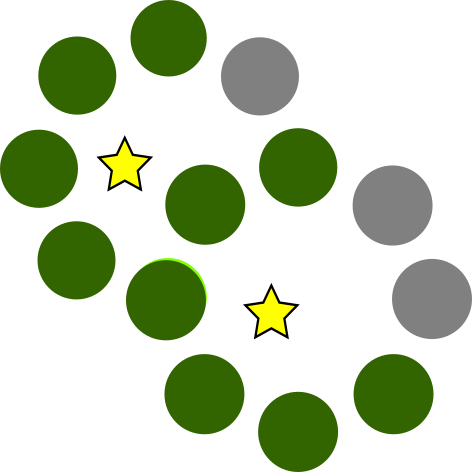
\includegraphics[scale=0.12]{../img/favicon.png}\\
{\huge Temporal Issue Tracking System\\}
{\Large User Manual}
\end{center}
\vfill
\newpage
\tableofcontents
\newpage
\setcounter{page}{3}
\pagenumbering{arabic}
\section{Requirements}
\subsection{Functional}
\begin{enumerate}[label=\textbf{FR\arabic*}]
    \item
    \item
\end{enumerate}
\subsection{Non-functional}
\subsection{Implementation}
\section{Pages}
\subsection{Login}
The first page user sees is the login page. The page consists of the login form and the button, leading to the signup page (in case the user does not have an account yet).
\begin{figure}[H]
    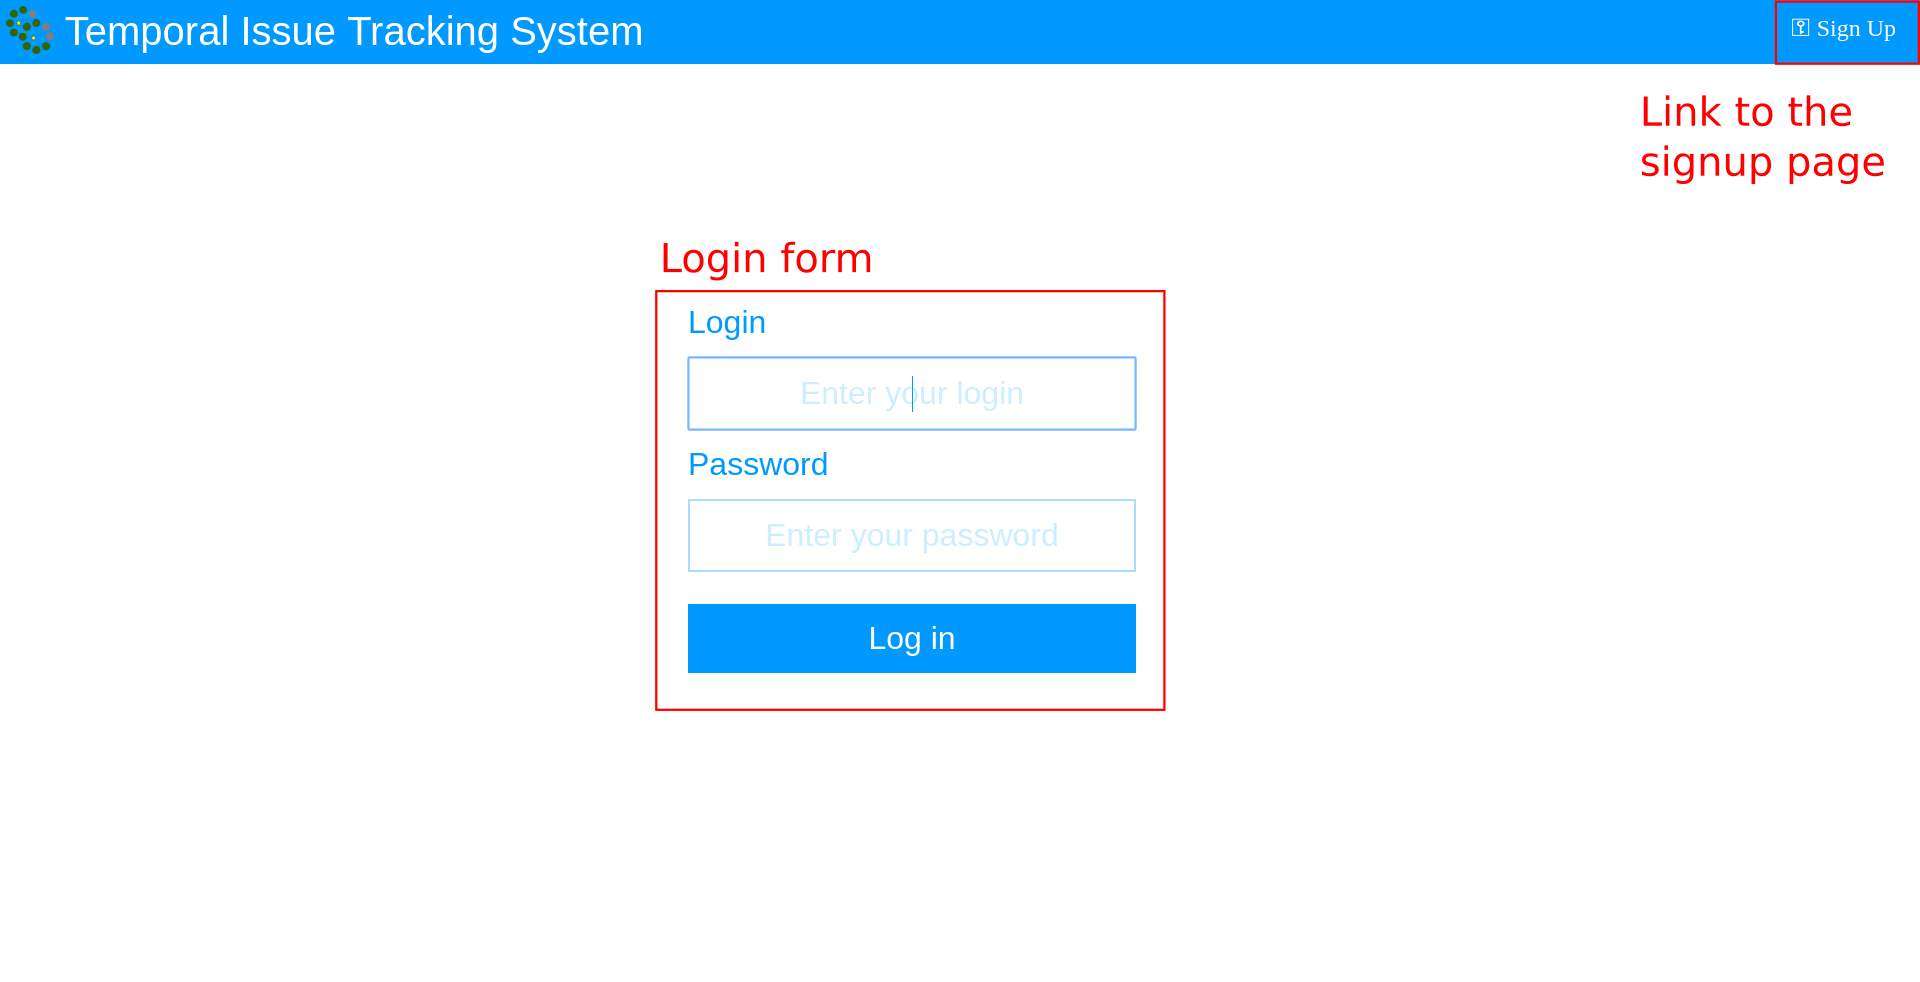
\includegraphics[width=\textwidth]{img/login.png}
    \caption{Login page}
\end{figure}
The login form consists of the labelled input fields for the login and password and the button that submits entered credentials when it's clicked. In order to improve user experience, user can log in using just keyboard for the login field is focused immediately after page is loaded and then one can switch to the password field pressing Tab (Shift-Tab to switch back) and submit the form by pressing Enter. After the field loses focus, it is pre-validated against the general rules, applicable to login and password (login should start with a letter and contain only alphanumeric characters, password should not be shorter than 5 characters) and it is styled according to the validation result. If validation fails, an information message is shown. On form submit all the fields are validated simultaniously.
\begin{figure}[H]
    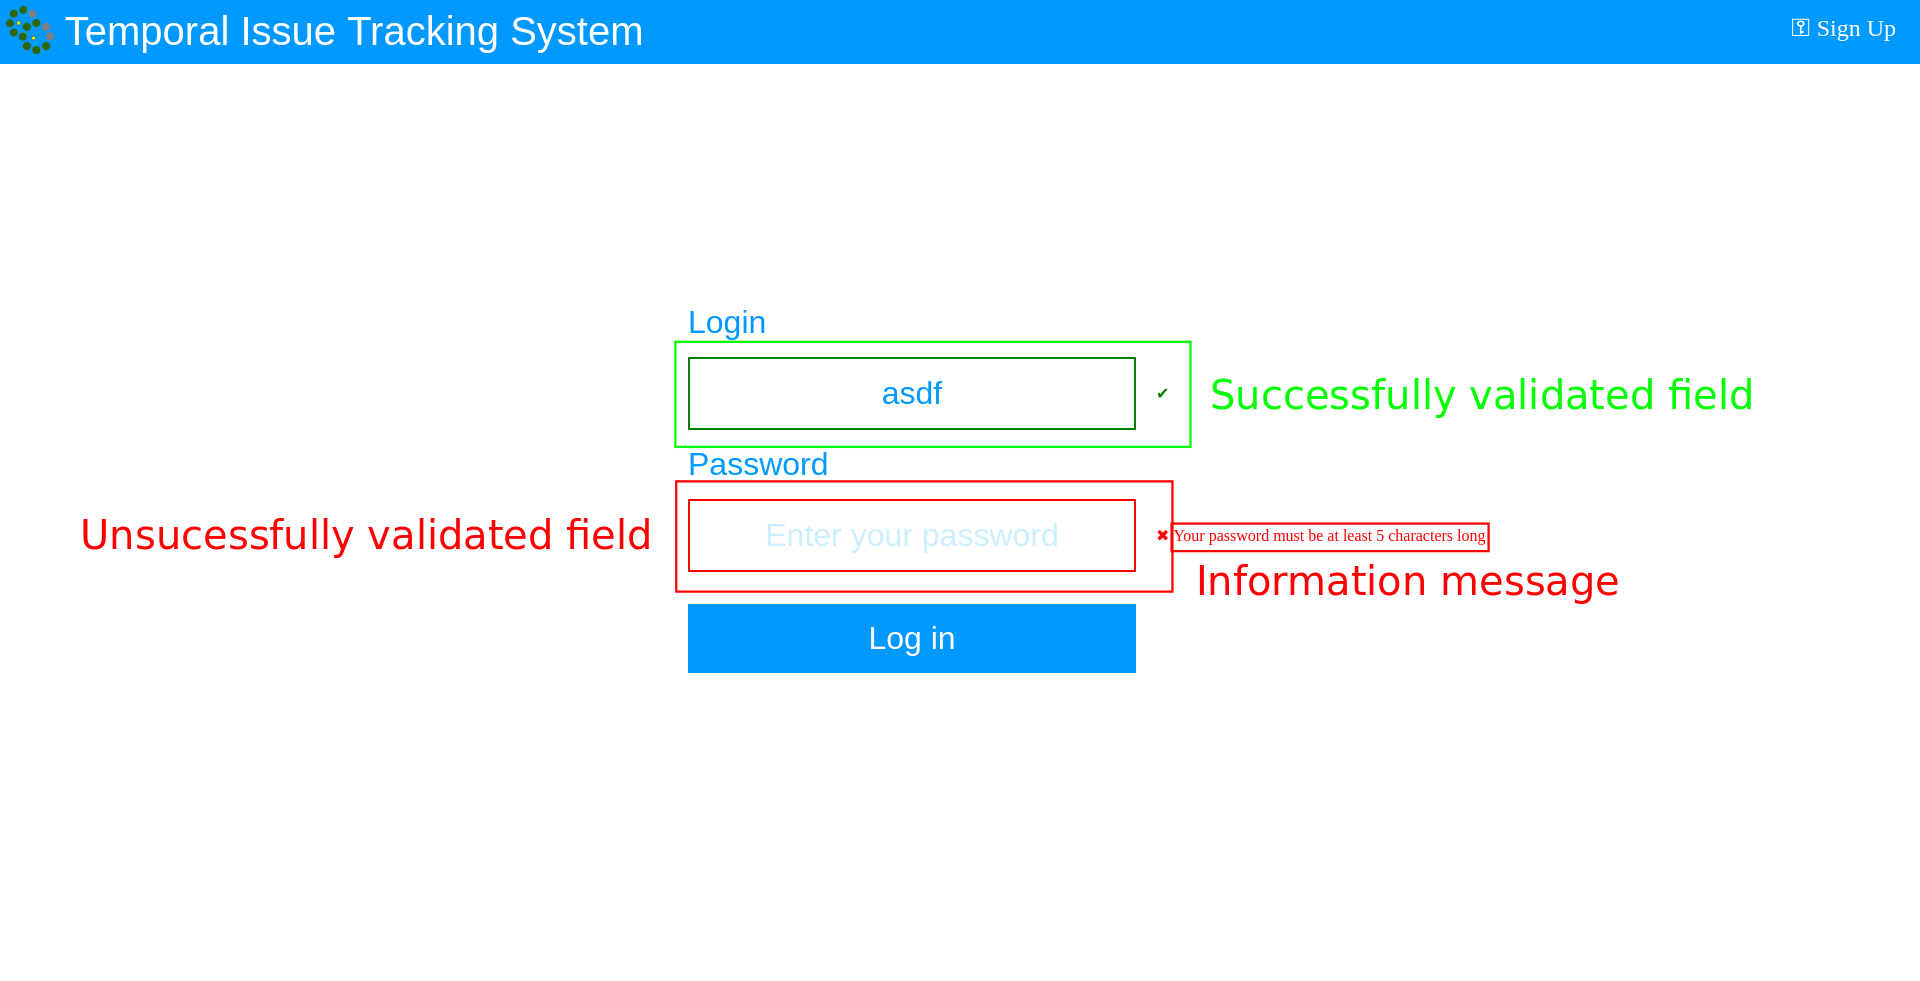
\includegraphics[width=\textwidth]{img/loginvalidation.png}
    \caption{Input pre-validation}
\end{figure}
On form submit (in case field pre-validation succeeded) credentials are being checked and if they are correct, the user is redirected to the home page. Otherwise an information message is shown and password field is erased.
\begin{figure}[H]
    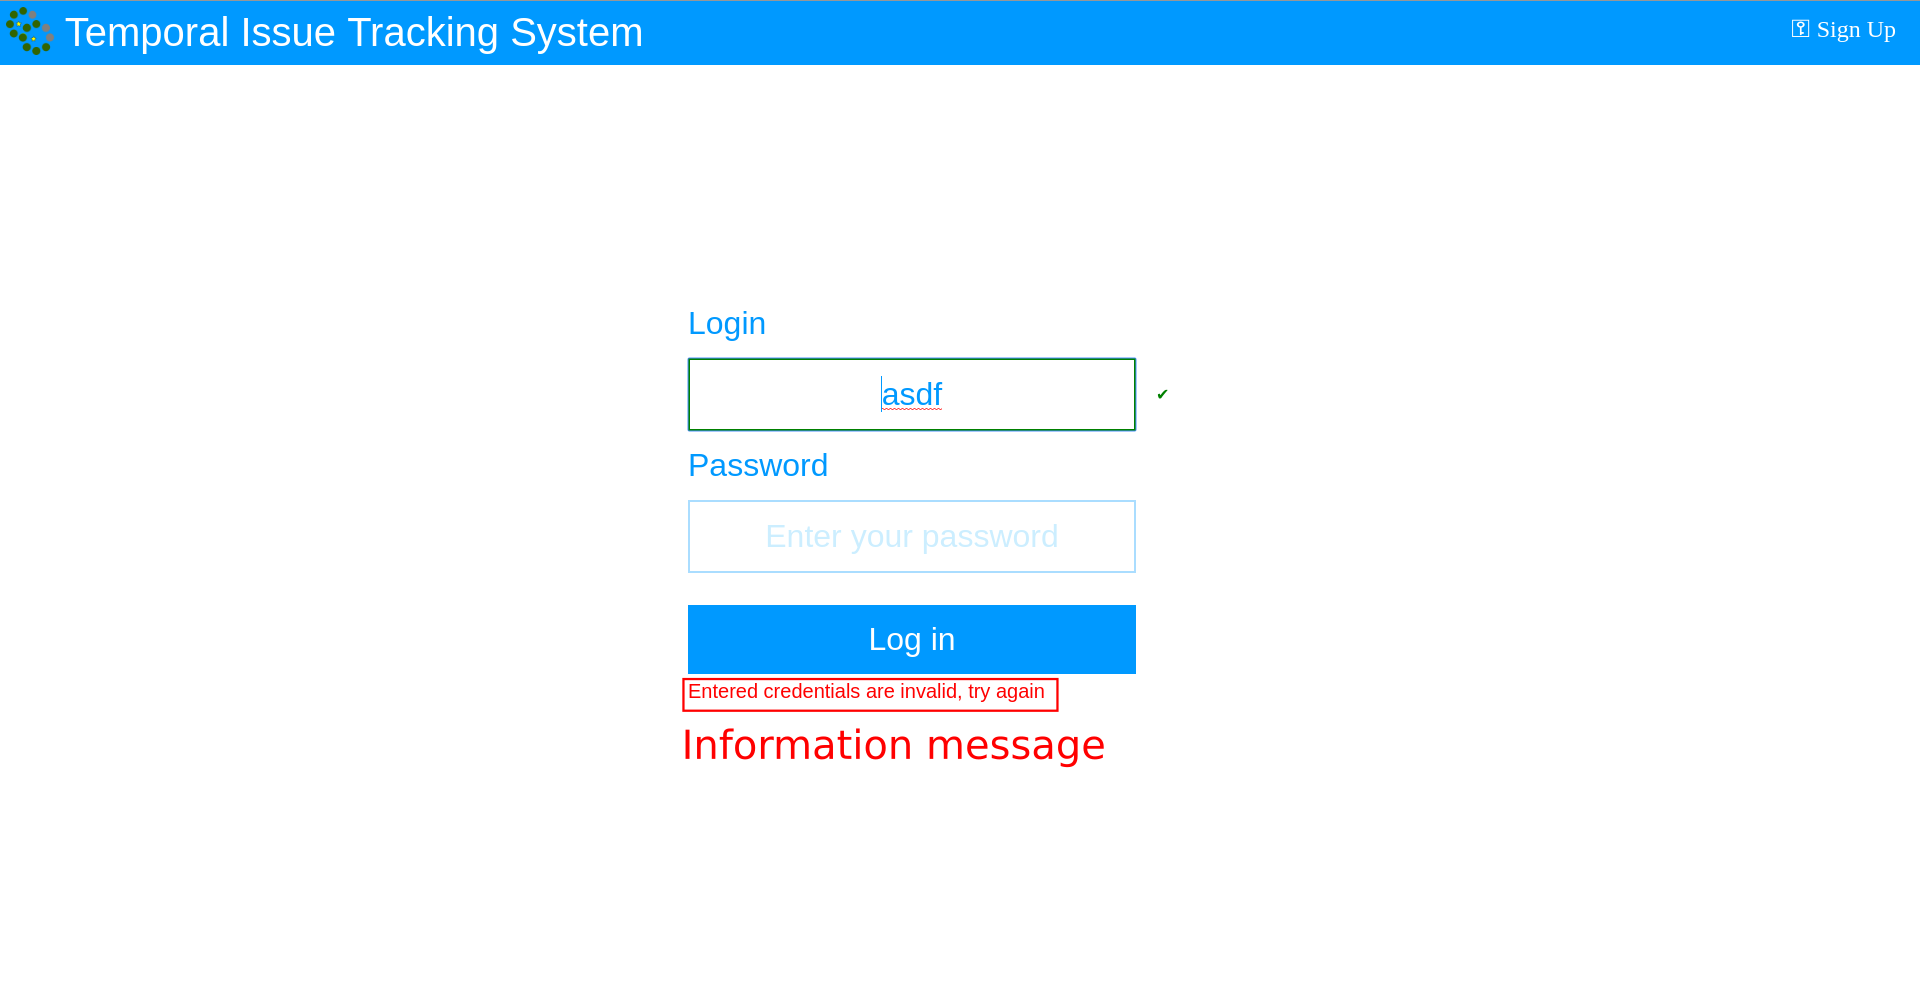
\includegraphics[width=\textwidth]{img/loginfailed.png}
    \caption{Login failed due to incorrect credentials}
\end{figure}
\subsection{Signup}
Signup page is similar to the login page but differs in the contents of the form. Signup form contains the following fields: name, login, password and confirmation. Pre-validation rules are the same for the username and password, name is not validated and pasword confirmation is checked against the password (if the values match). The button in the top-rigth corner leads to the login page.
\begin{figure}[H]
    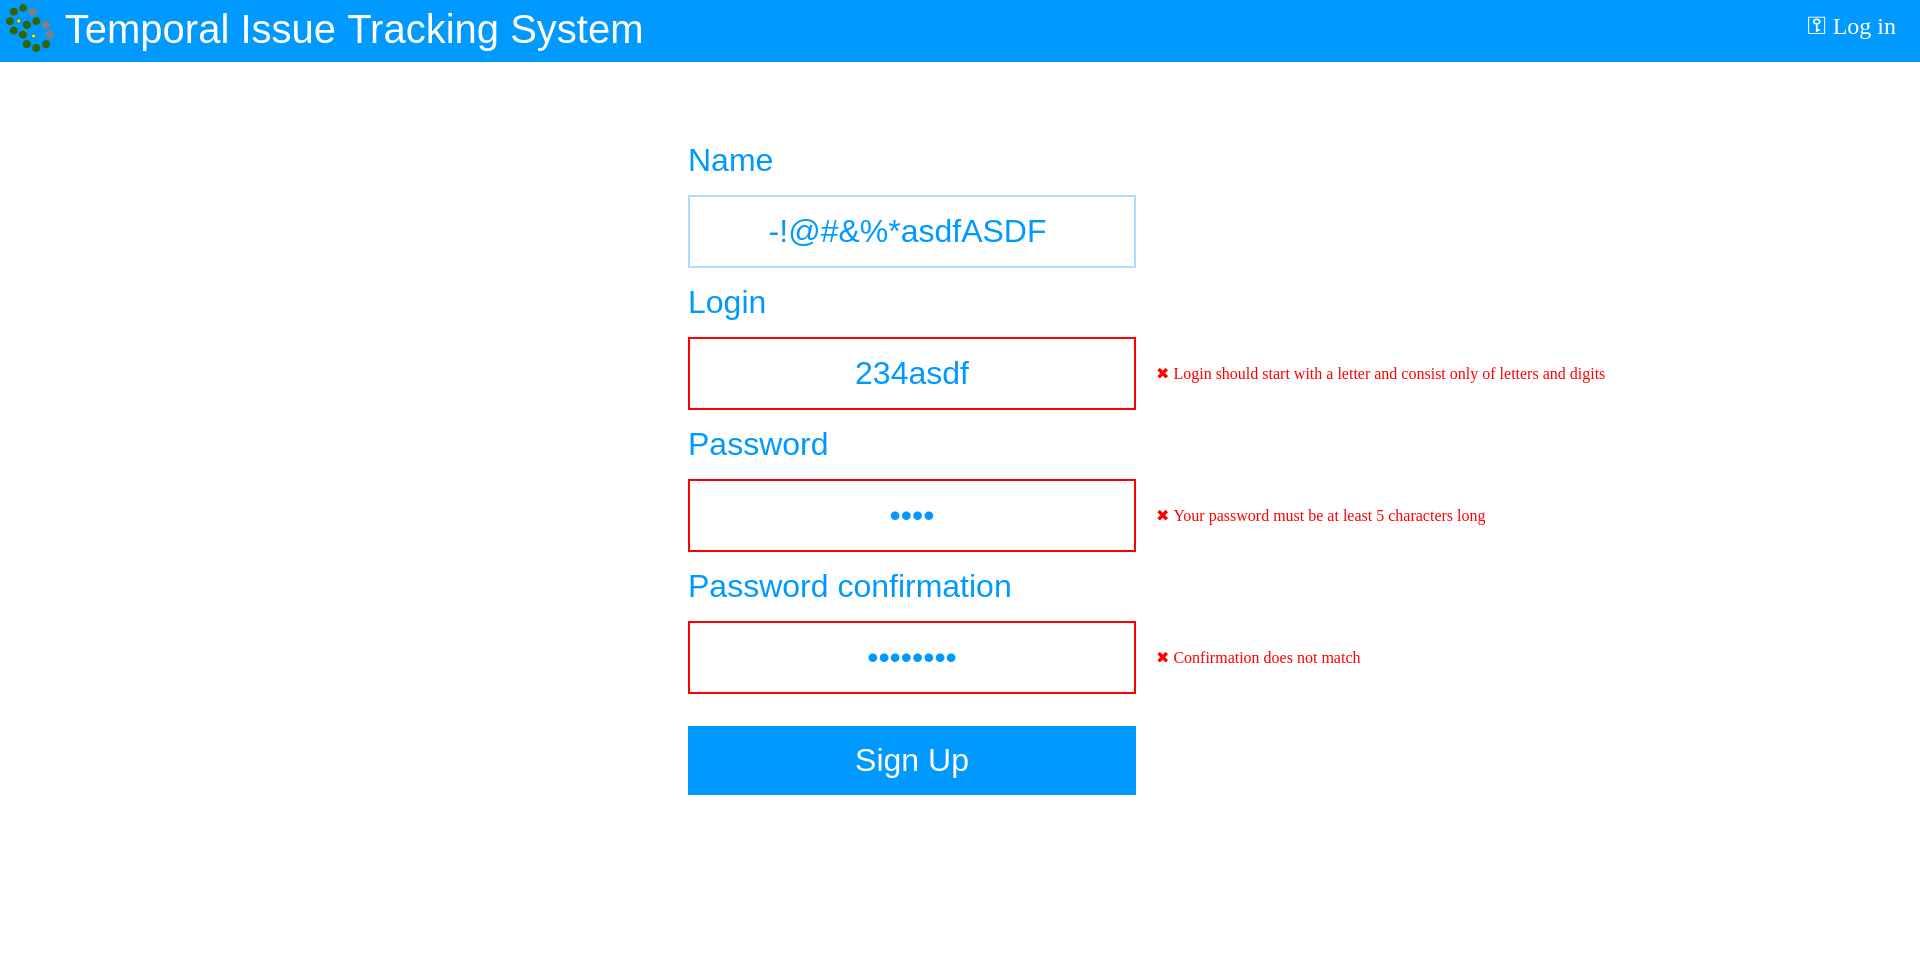
\includegraphics[width=\textwidth]{img/signup.png}
    \caption{Signup page}
\end{figure}
On signup the entire form is pre-validated and (in case of success) the login is checked for availability and the result is shown as an information message and passwords fields are erased. In case of success other fields are erased too.
\begin{figure}[H]
    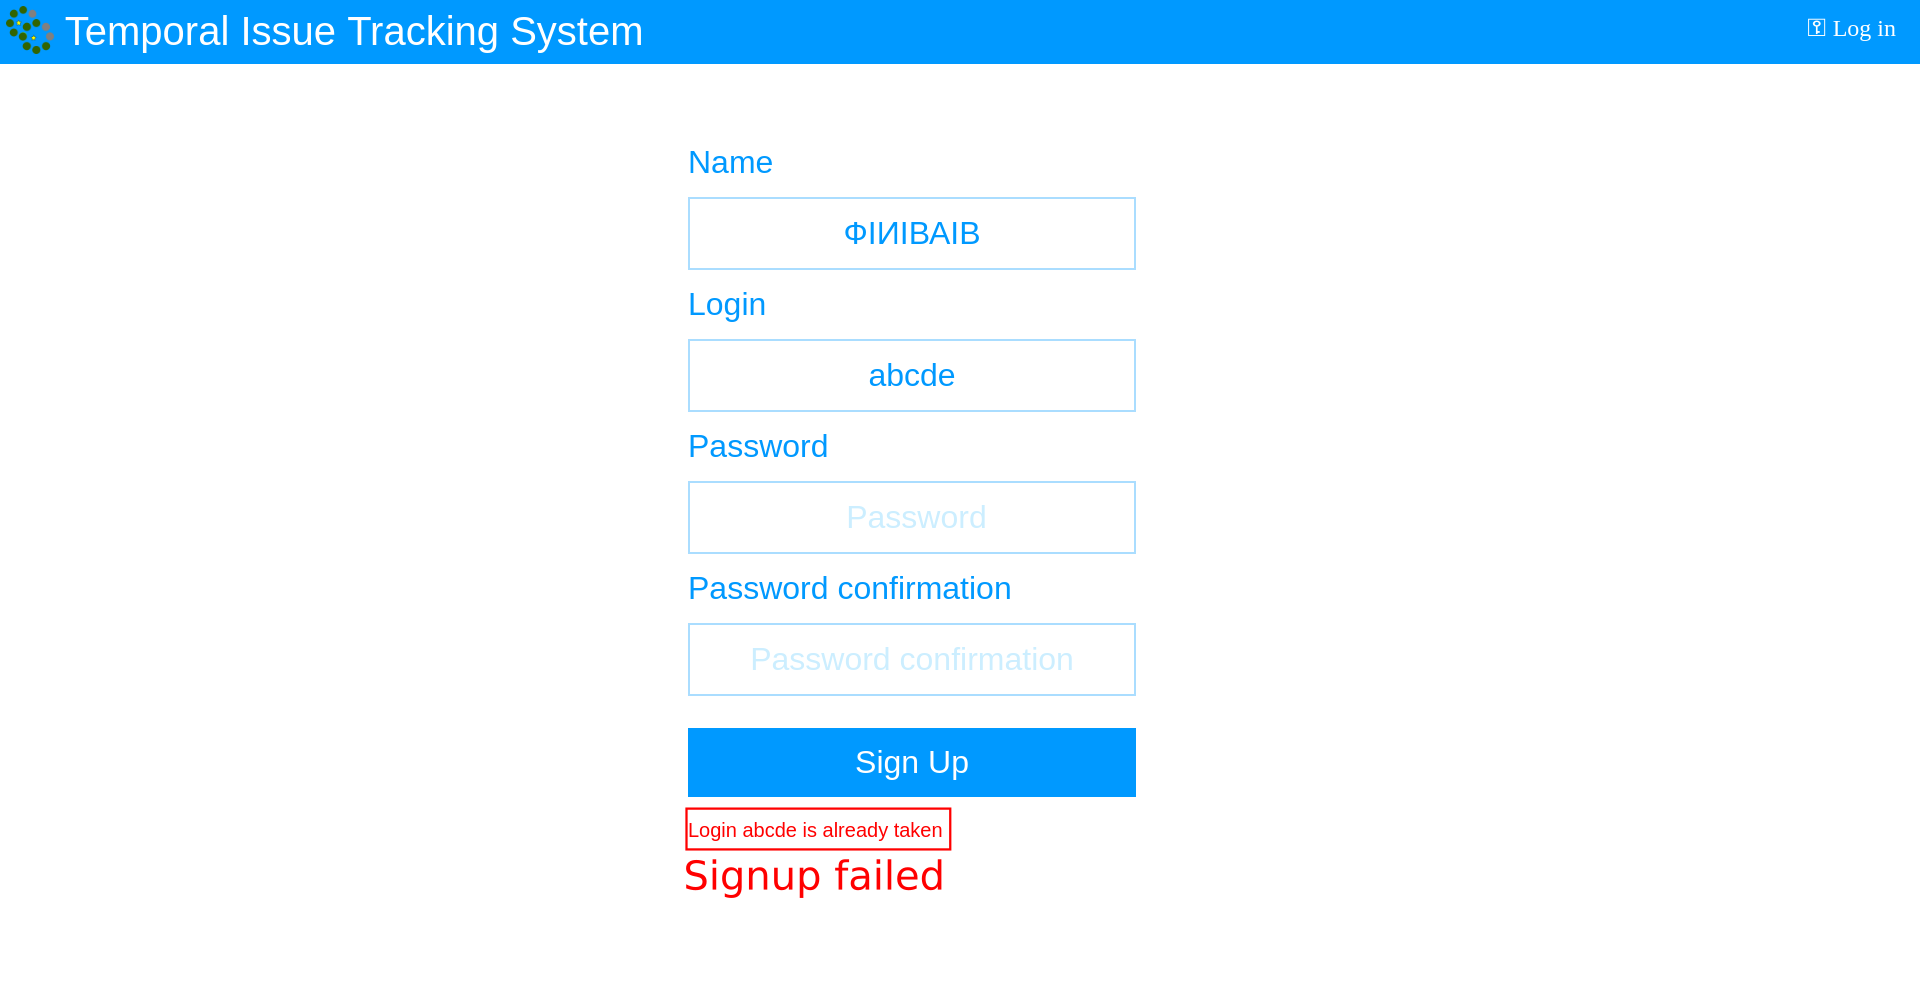
\includegraphics[width=\textwidth]{img/signupfailed.png}
    \caption{Signup failed due to login being already taken}
\end{figure}
\begin{figure}[H]
    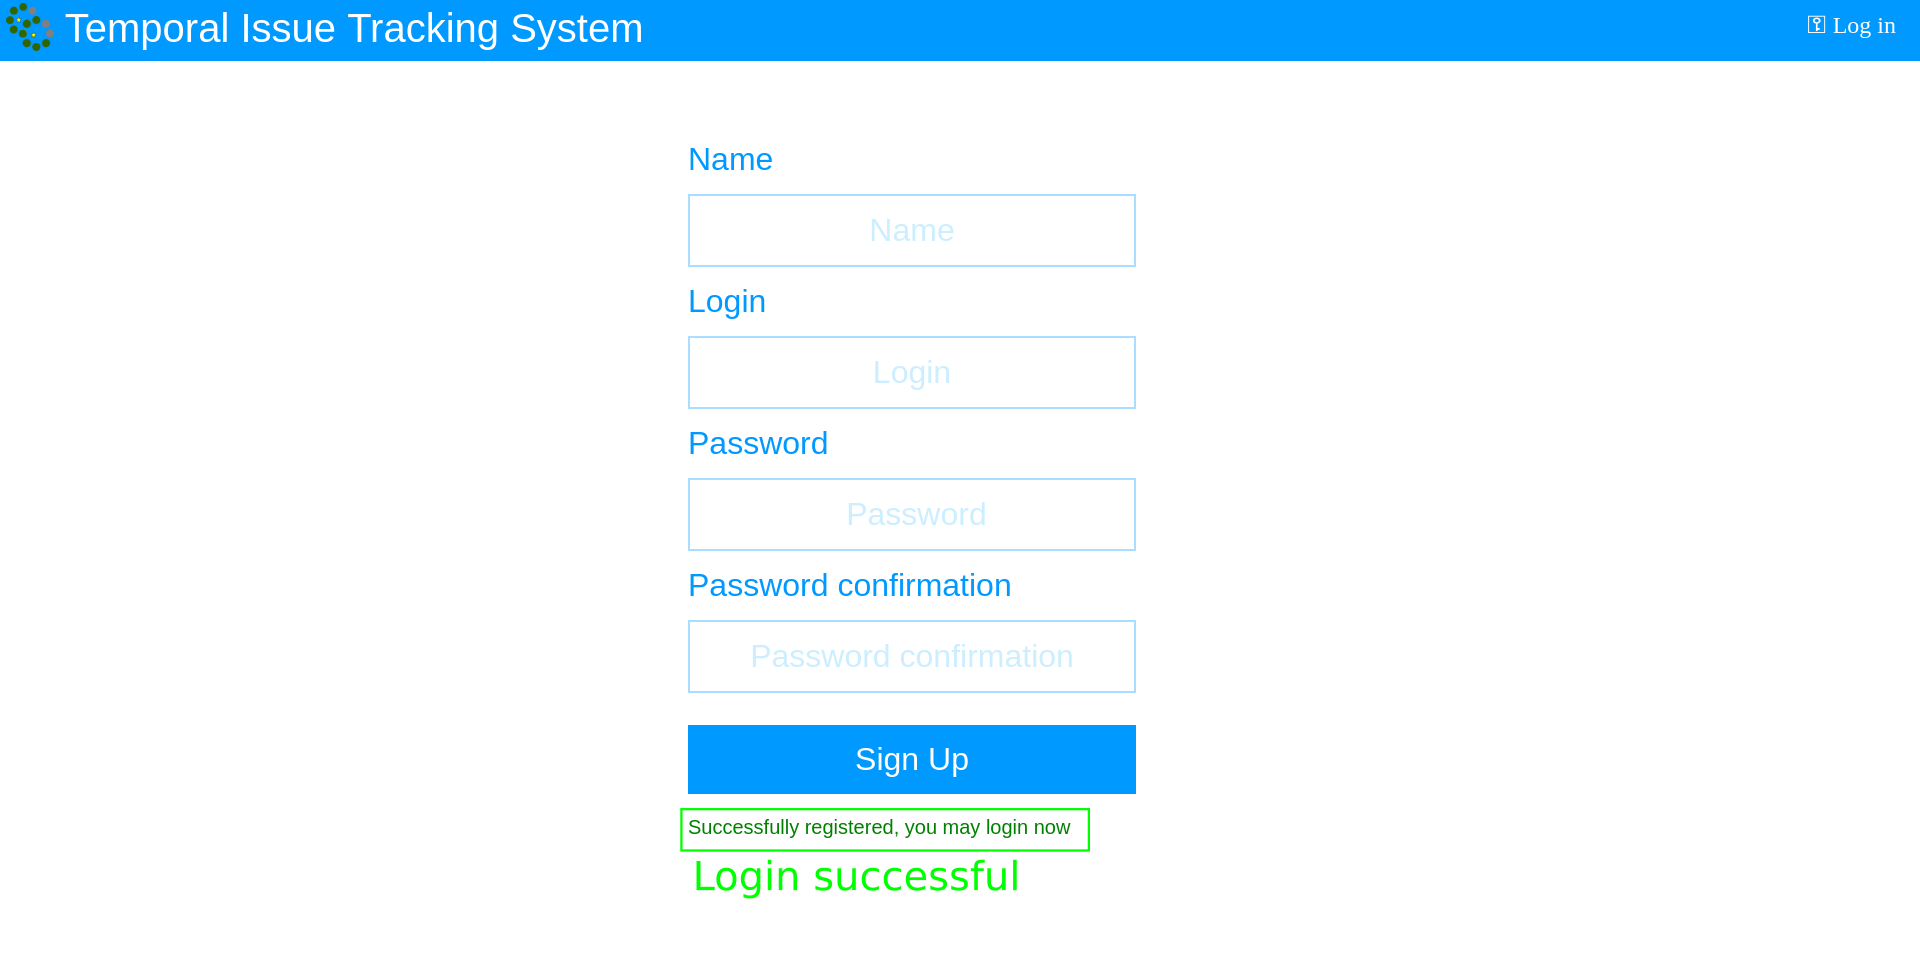
\includegraphics[width=\textwidth]{img/signupsuccessful.png}
    \caption{Signup succeeded}
\end{figure}
\subsection{Home}
After user is logged in, the home page is shown. The header (which is virtually the same throughout the entire application) serves as a navigation menu, shows the name of the current user (and login in the tooltip) and lets the user to log out.\\
In the main part of the page the application title and welcome message is shown above the list of the tasks, requiring user's attention the most. Task entries will be discussed later in this Manual.
\begin{figure}[H]
    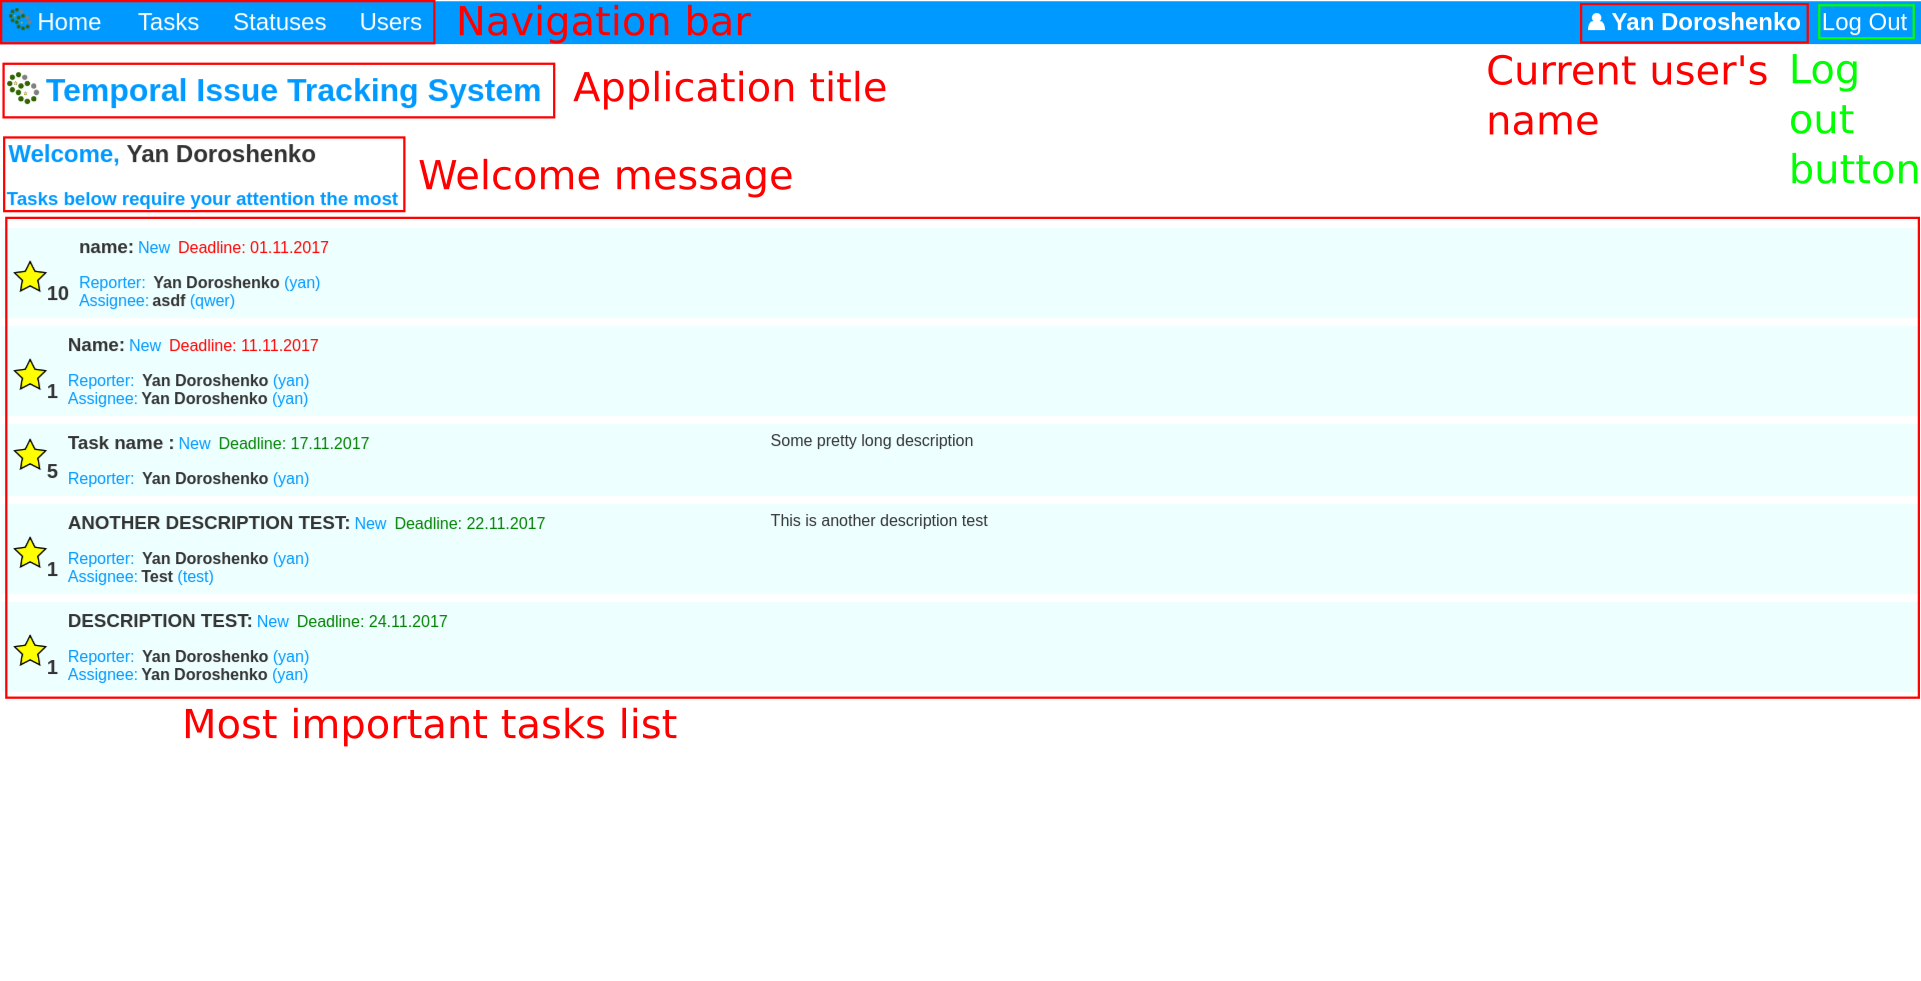
\includegraphics[width=\textwidth]{img/home.png}
    \caption{Home page}
\end{figure}
\subsection{Tasks}
\subsubsection{List}
Task list can be accessed using the navigation bar in the header. This page shows the paginated list of all the tasks. The number of all the tasks is shown in the bottom-right angle together with the indicator, which entries are show on the current page. Bottom-left corner accomodates page navigation buttons. Tasks can be searched by name and description using the filter in the header. There is also a button, redirecting to the task creation page, in the header.
\begin{figure}[H]
    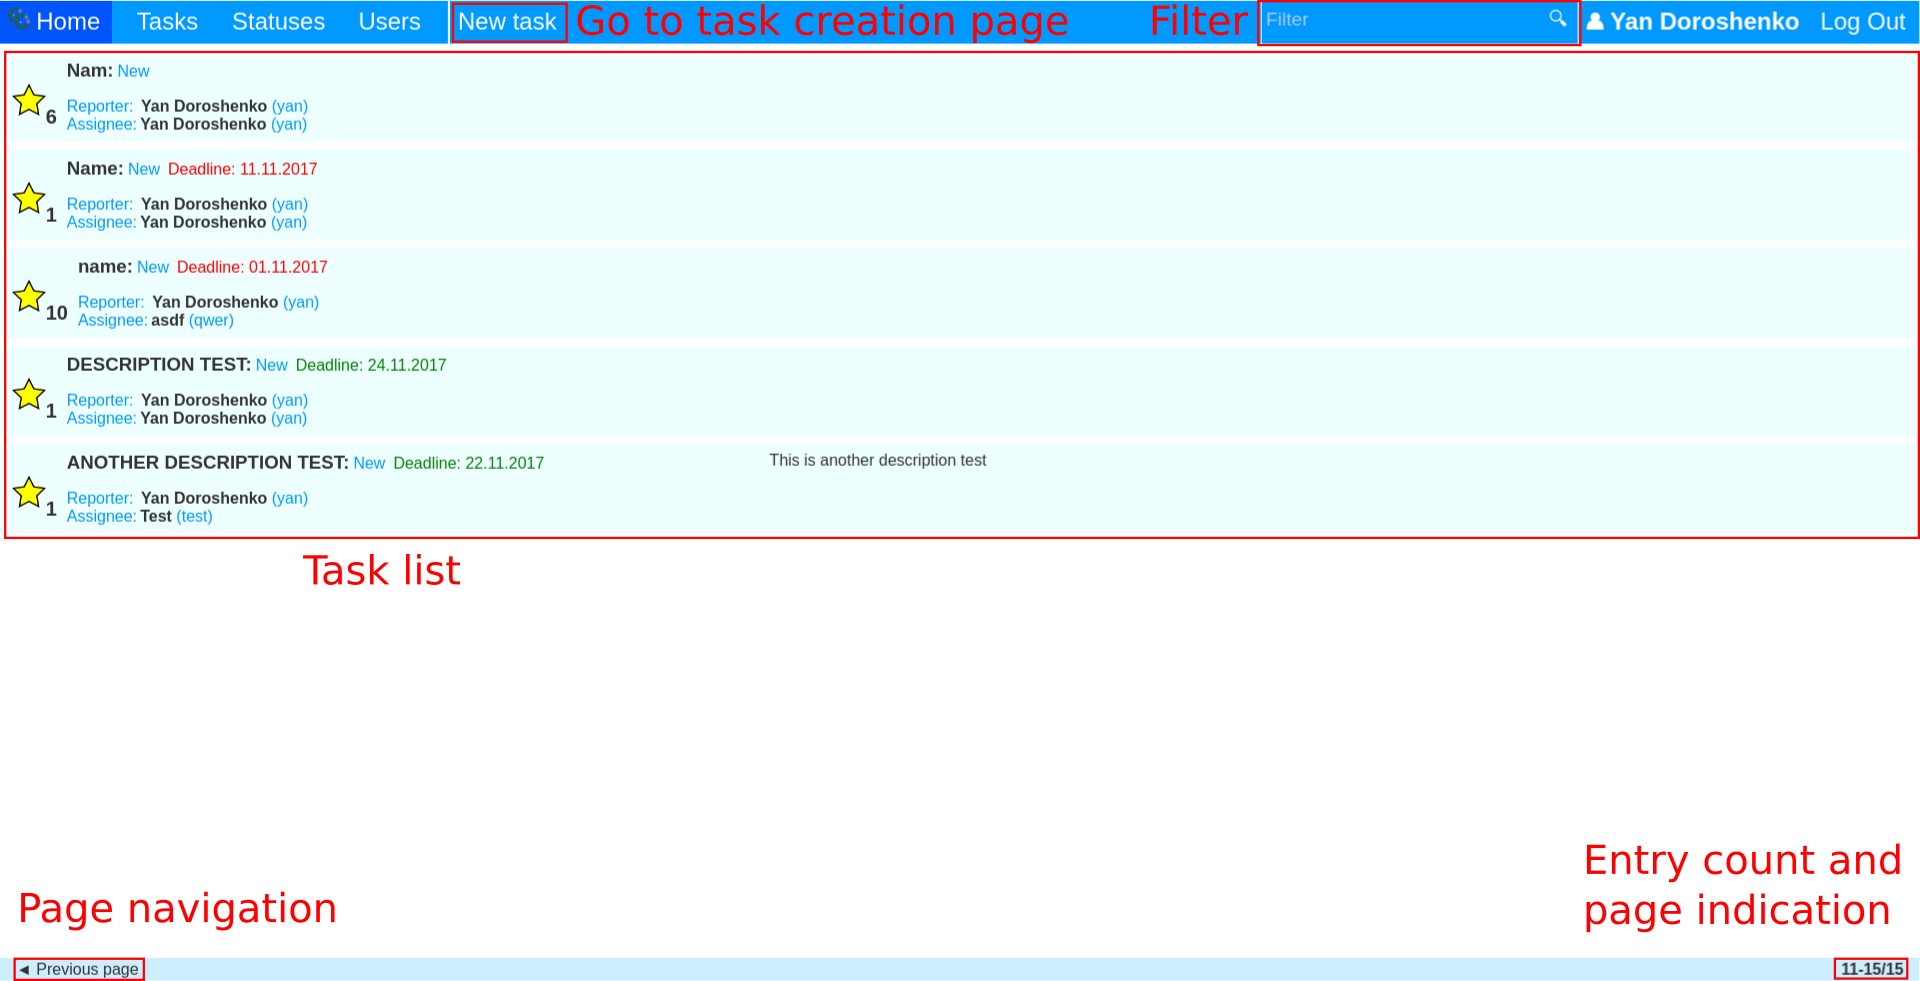
\includegraphics[width=\textwidth]{img/tasks.png}
    \caption{Task list page}
\end{figure}
Each task entry contains most information about the task: name, priority (1 to 10, 1 is the most important), description, status icon and title, deadline (shown in red if passed), reporter's and assignee's name and login. Clicking on the entry redirects to the task details page.
\begin{figure}[H]
    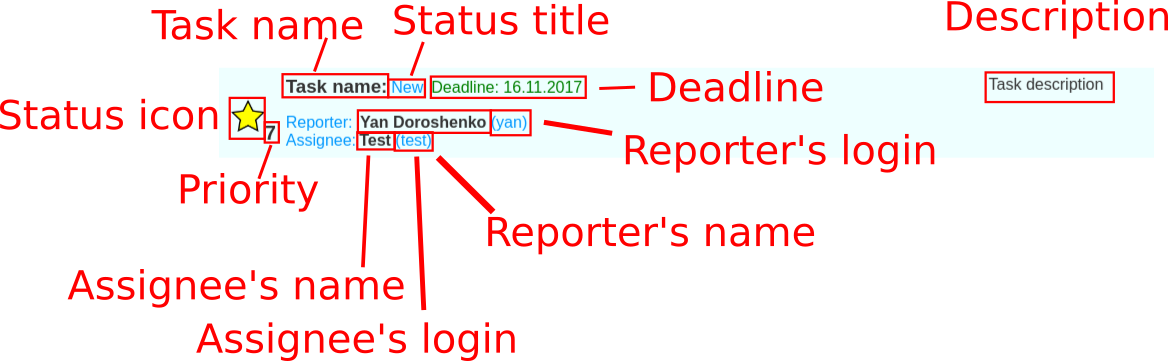
\includegraphics[width=\textwidth]{img/task.png}
    \caption{Task entry}
\end{figure}
\subsubsection{Creation}
Task creation page can be accessed from the task list page via the button in the header. It contains the form, letting the user to provide the details for the new task. There are only two required fields - priority and task name. All the other fields are optional. Task is created by clicking the "Create" button.
\begin{figure}[H]
    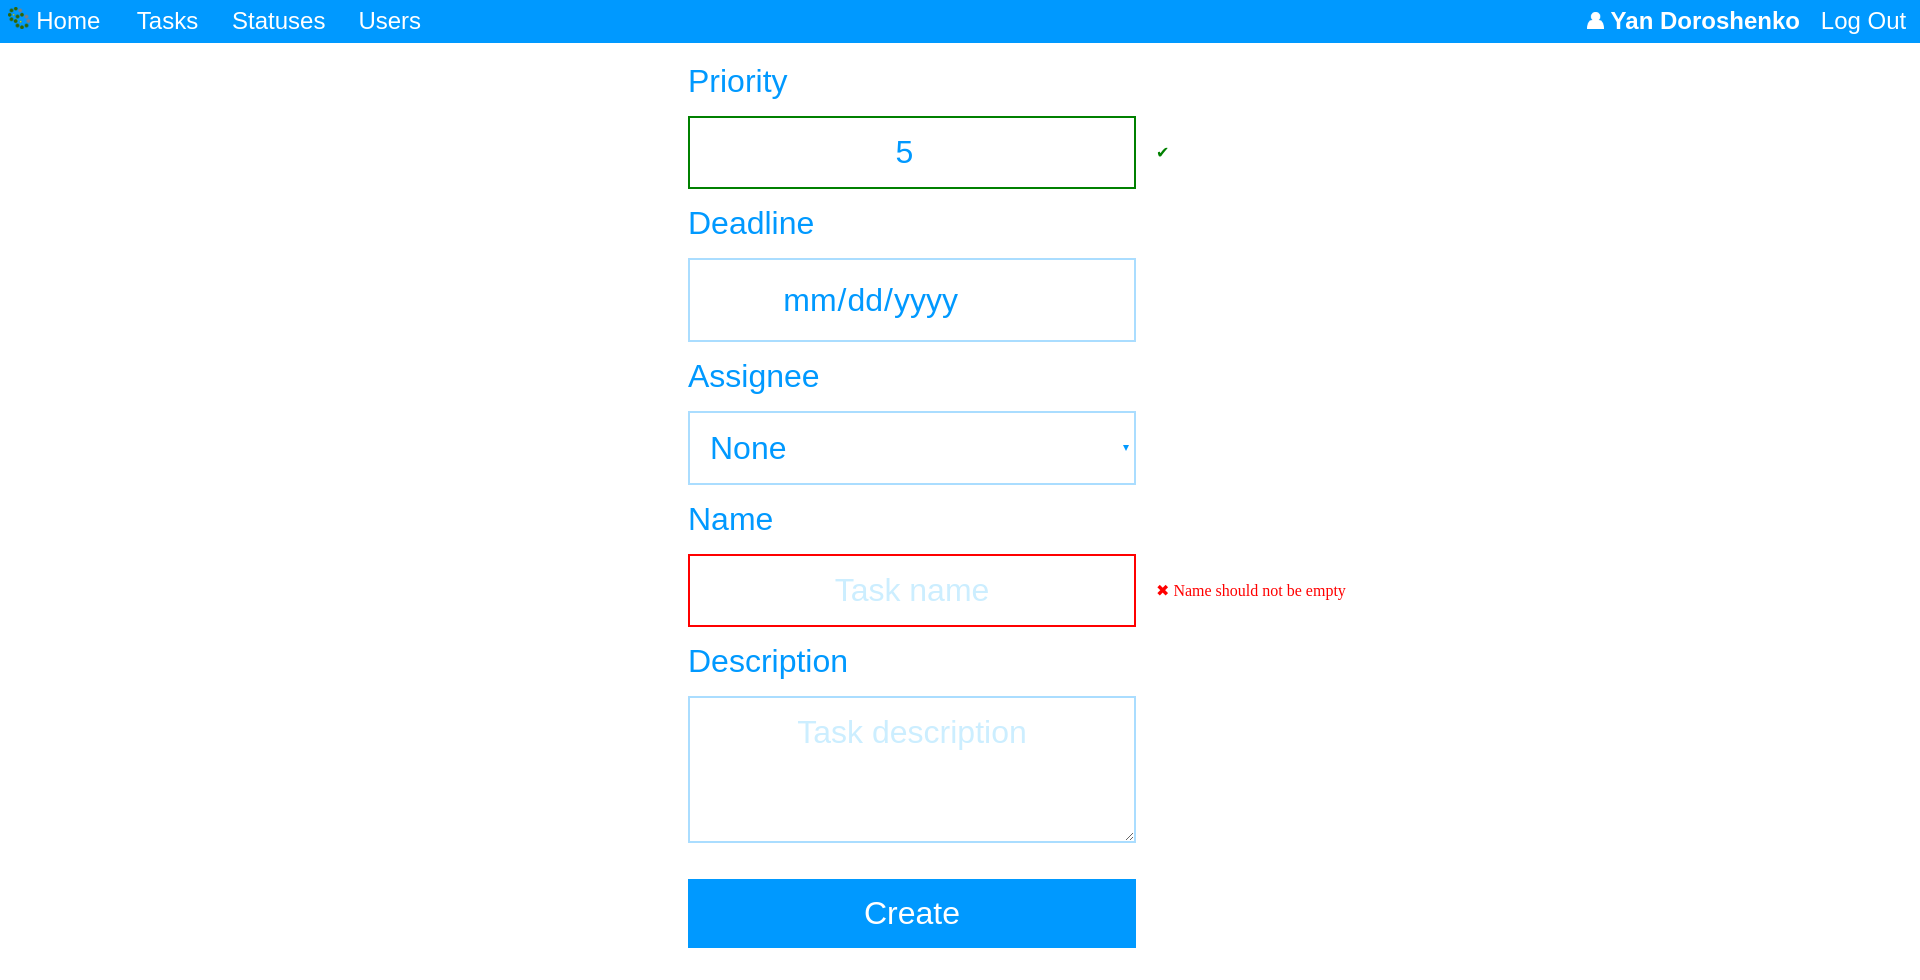
\includegraphics[width=\textwidth]{img/createtask.png}
    \caption{Task creation page}
\end{figure}
\subsubsection{Details}
Task details page shows the task details and allows the reporter to edit the task.
\begin{figure}[H]
    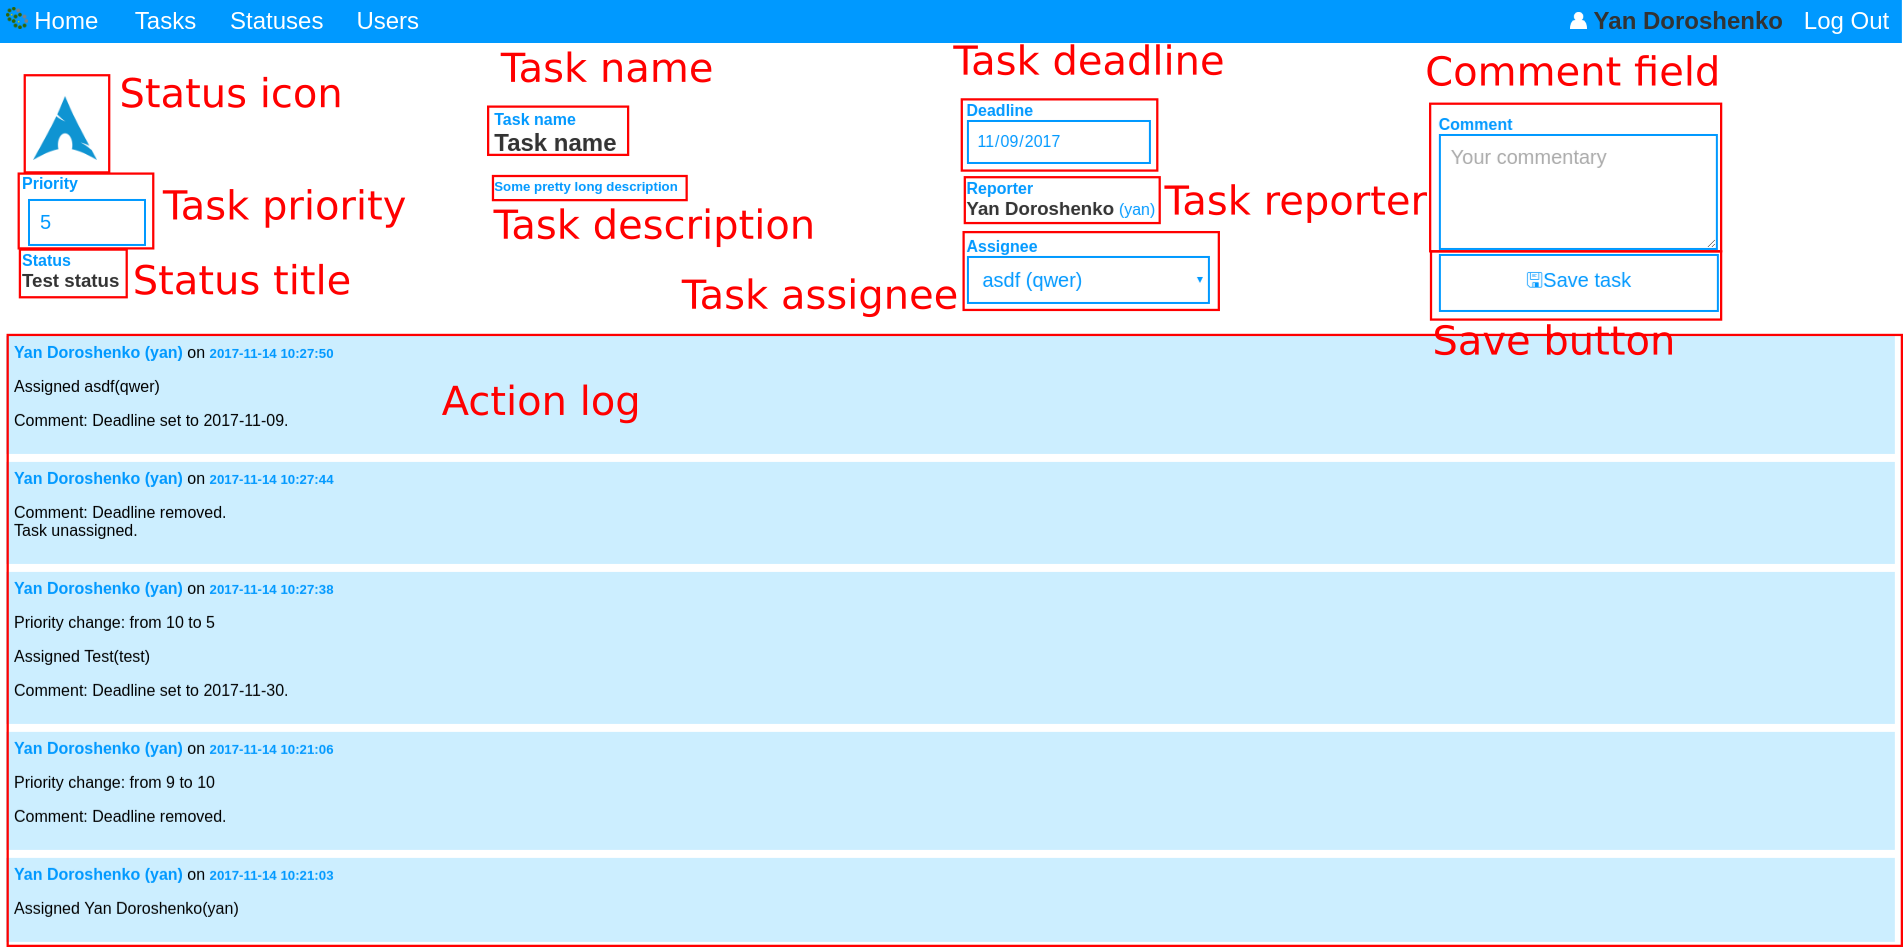
\includegraphics[width=\textwidth]{img/taskdetails.png}
    \caption{Task details page}
\end{figure}
Comment field is for everyone to fill. Submitting a comment creates a log entry with a comment.\\
Reporter can edit priority, status, assign and unassign users, add, edit and remove deadline.\\
Assignee can change status.\\
Note: status can't be changed once task is assigned a final status.\\
Save button saves the changes, updates the task and creates an action log entry, containing all the changes made.\\
\begin{figure}[H]
    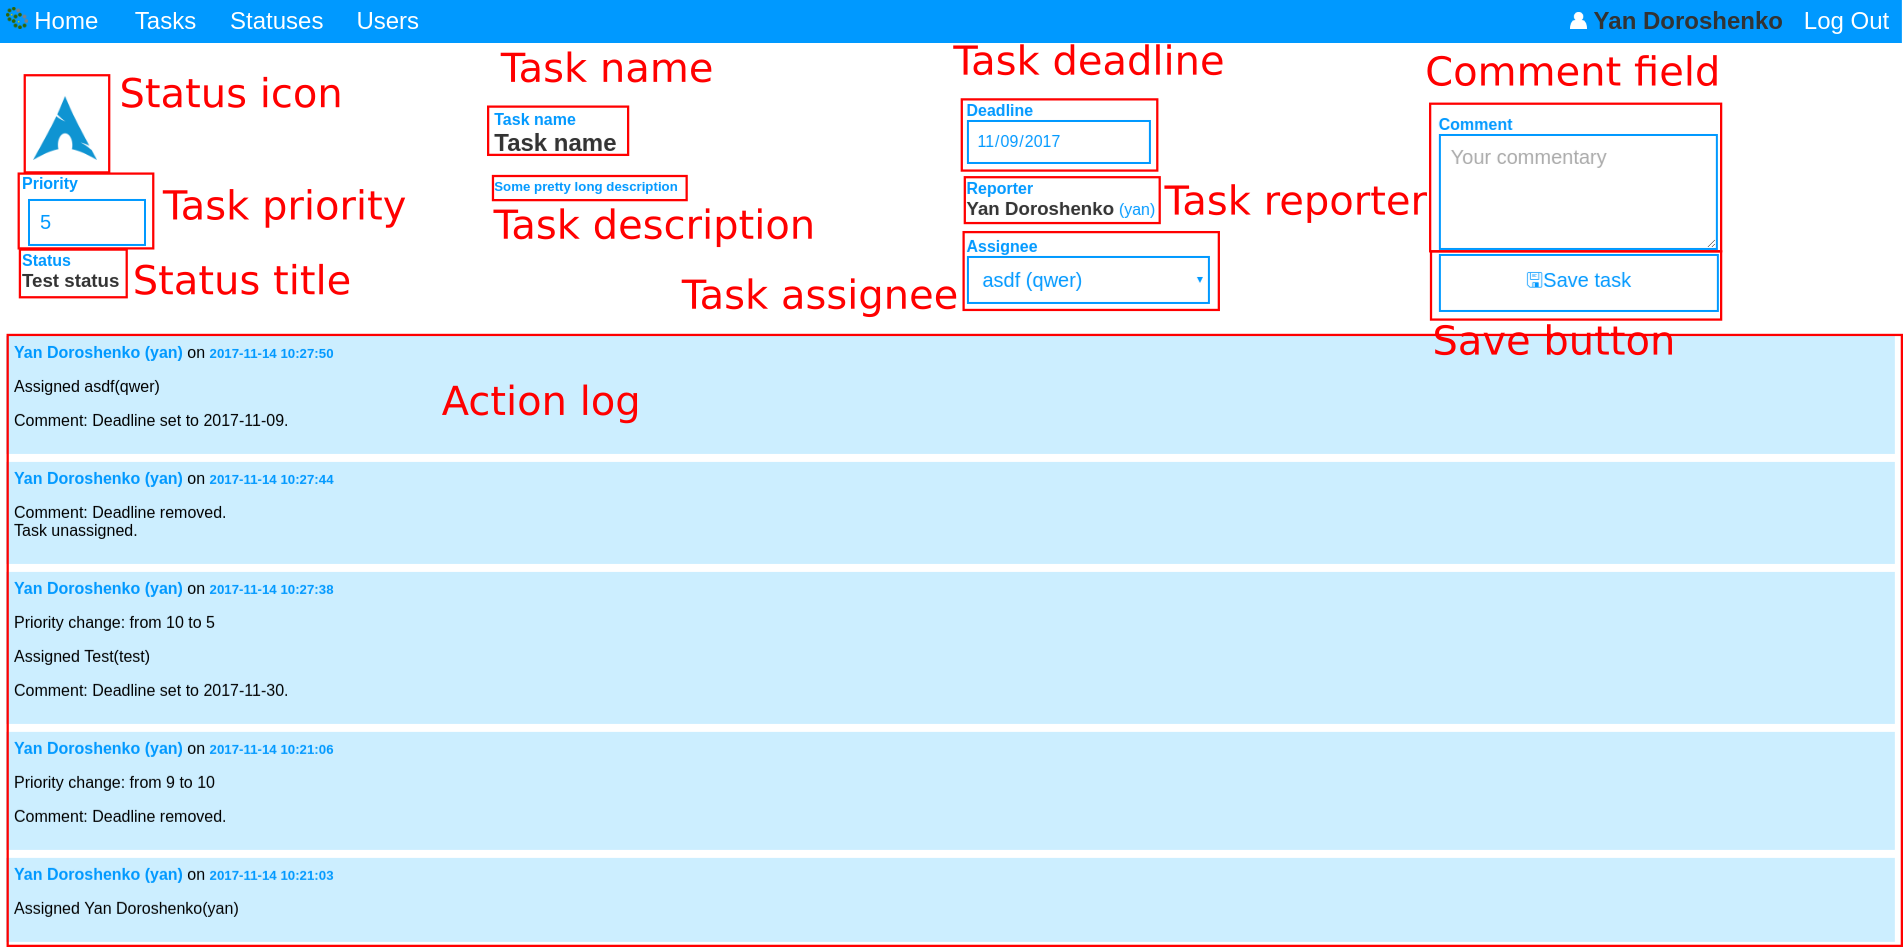
\includegraphics[width=\textwidth]{img/taskdetails.png}
    \caption{Task details page}
\end{figure}
Action log entry contains information about the user, performing the action, date and time when it was performed, description of all the changes, and a comment.
\begin{figure}[H]
    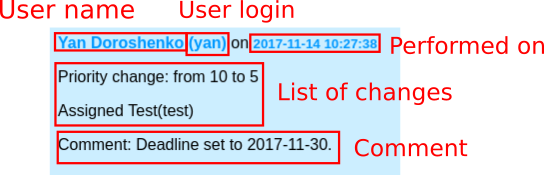
\includegraphics[width=\textwidth]{img/action.png}
    \caption{Action log entry}
\end{figure}
\subsection{Statuses}
\subsubsection{List}
The status list page can be accessed via the button in the header. It has the same paging, filtering and entry creation features as described before regarding the task list page.
\begin{figure}[H]
    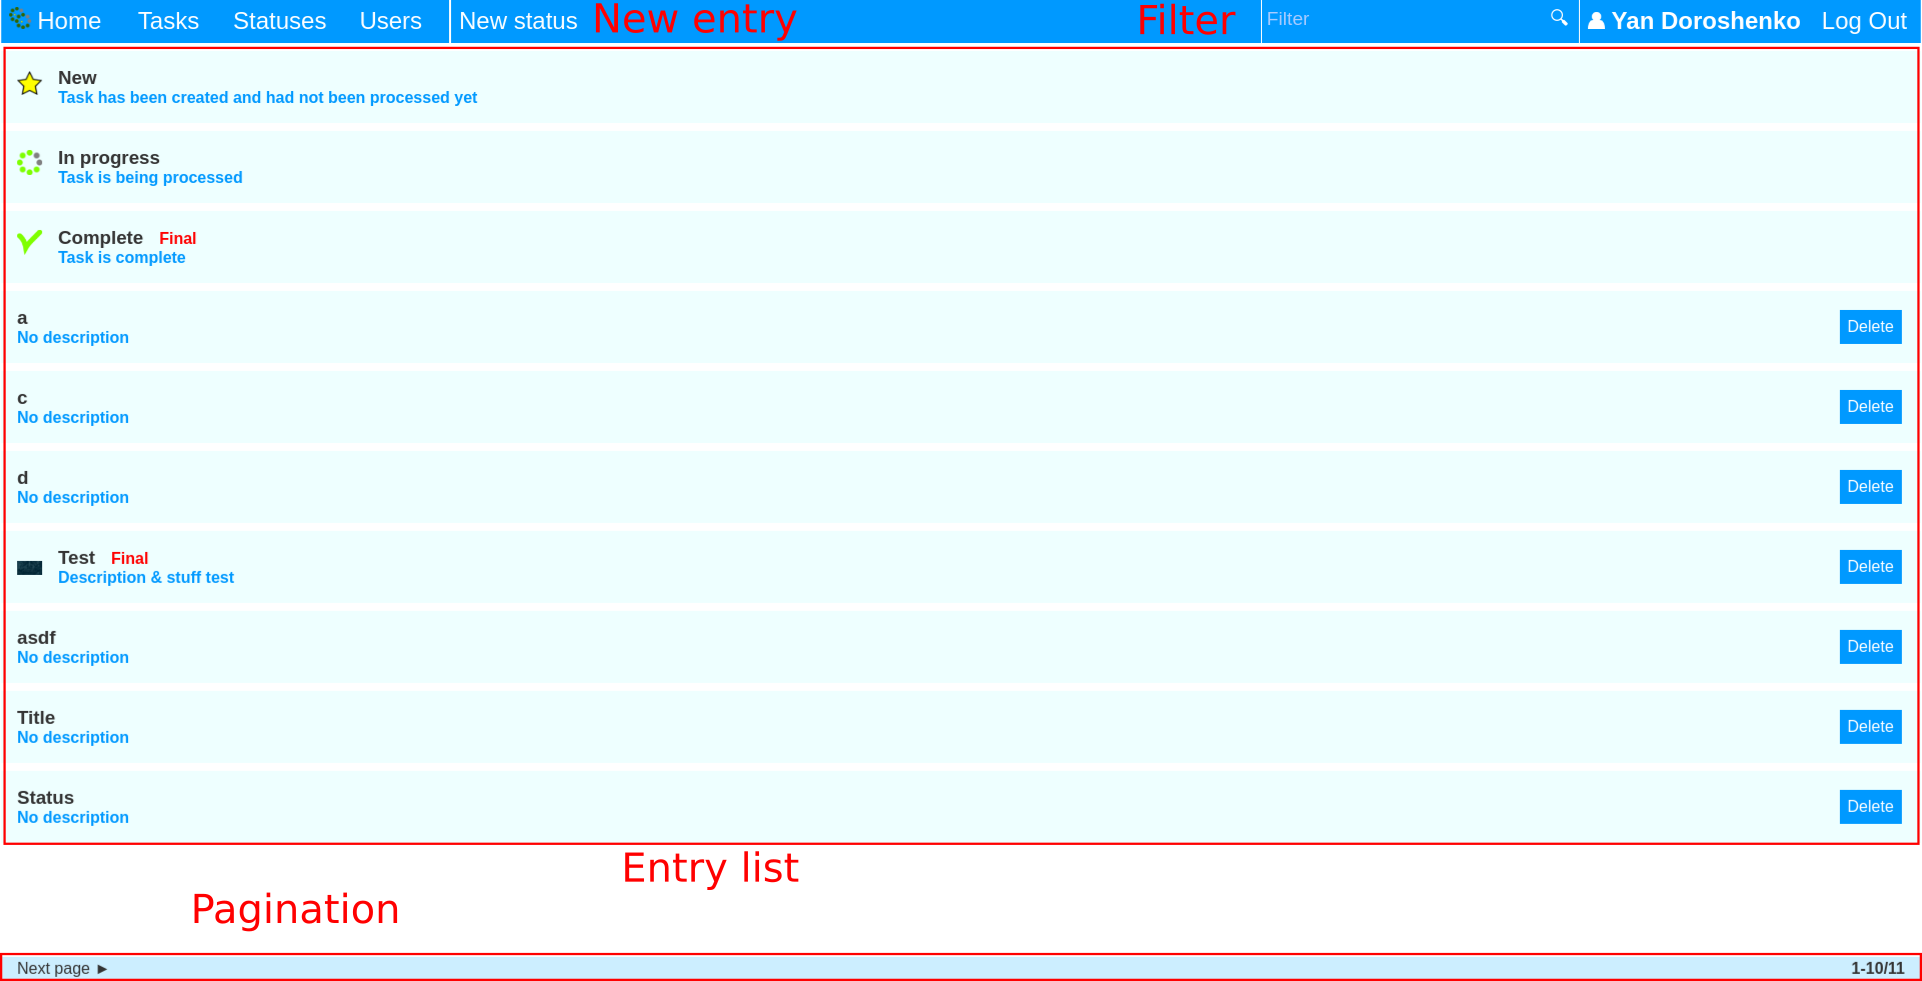
\includegraphics[width=\textwidth]{img/statuses.png}
    \caption{Status list page}
\end{figure}
Status entry contains all the information about the status (title, description, icon, whether the status is final) and enables deletion of the non-system statuses (system statuses are firmly set and can not be deleted).
\begin{figure}[H]
    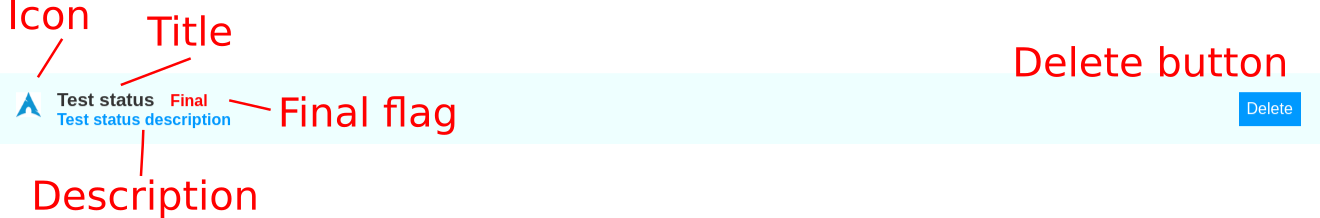
\includegraphics[width=\textwidth]{img/status.png}
    \caption{Status entry}
\end{figure}
When "Delete" button is clicked, status is checked for dependent tasks (task that had this status set at some point). If nothing is found, status is deleted and the list is refreshed. Otherwise, information message is shown.
\begin{figure}[H]
    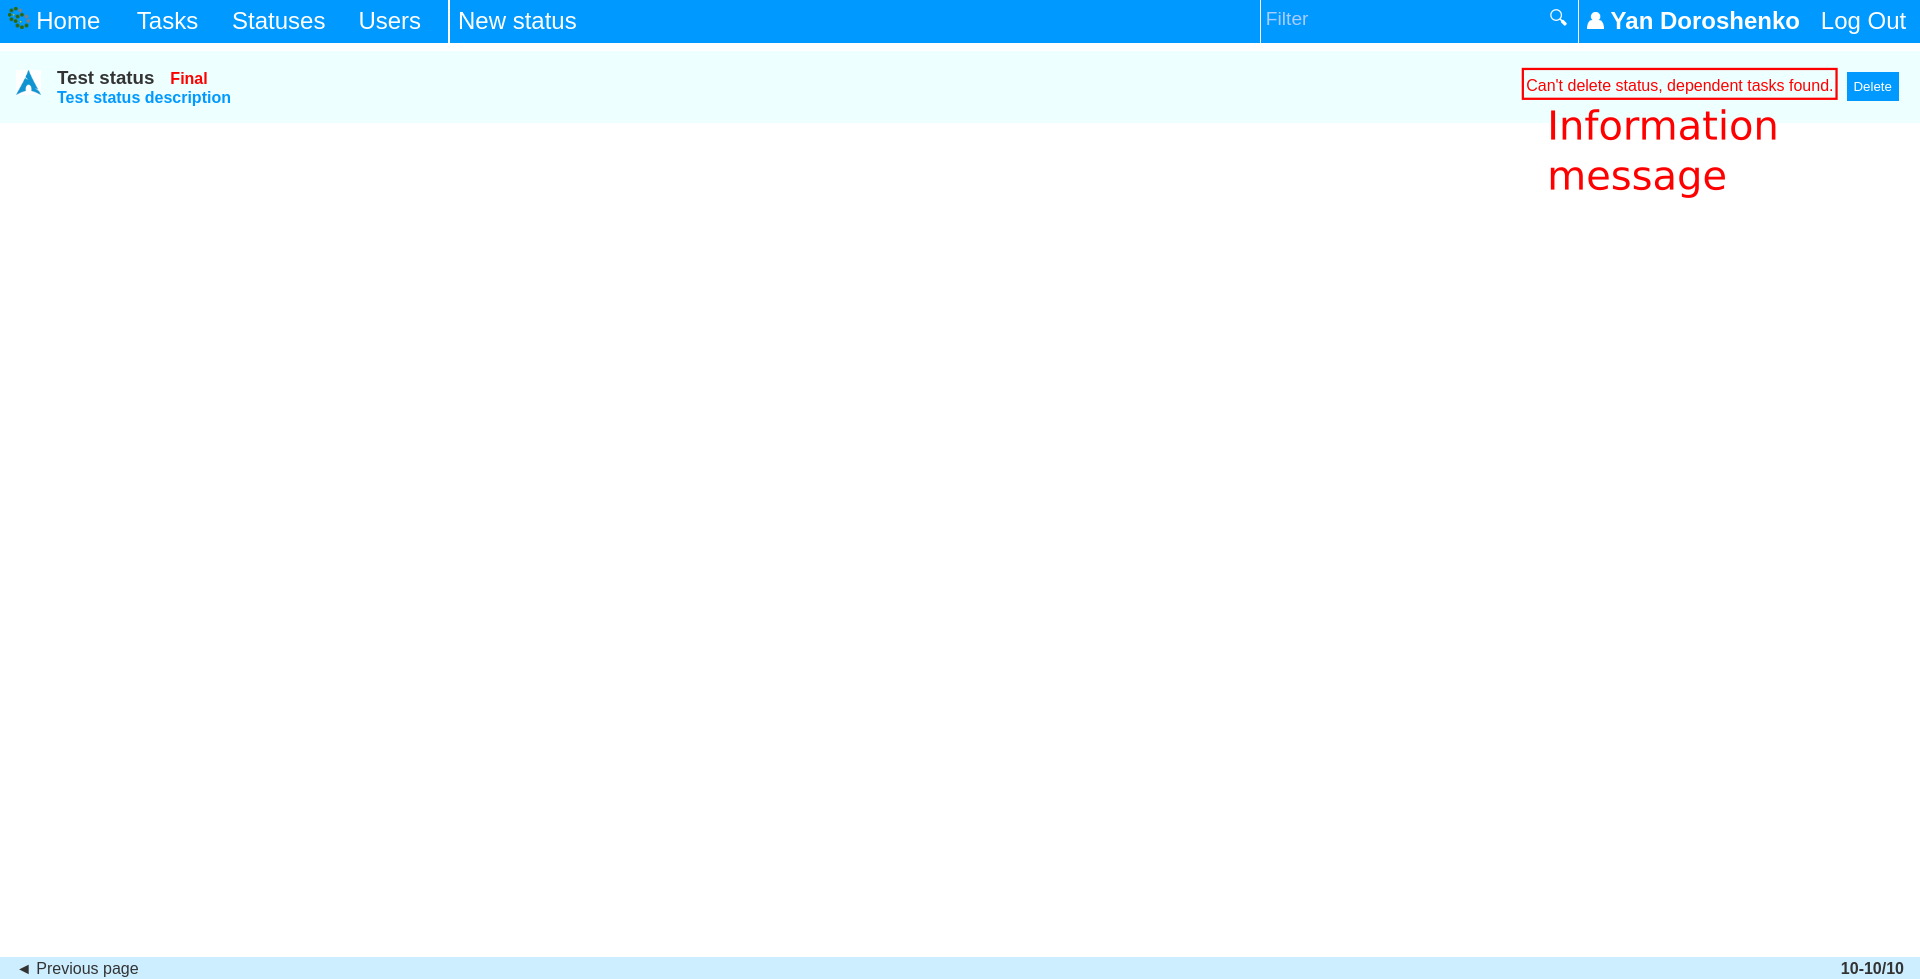
\includegraphics[width=\textwidth]{img/deletestatus.png}
    \caption{Status deletion failed}
\end{figure}
\subsubsection{Creation}
Status creation page can be accessed from the status list page via the button in the header. It contains the form, letting the user to provide the details for the new status. Title is required. Checking the "Final" checkbox means that the task's status can't be changed after this status is assigned. Icon upload file is checked to be a valid image file.
\begin{figure}[H]
    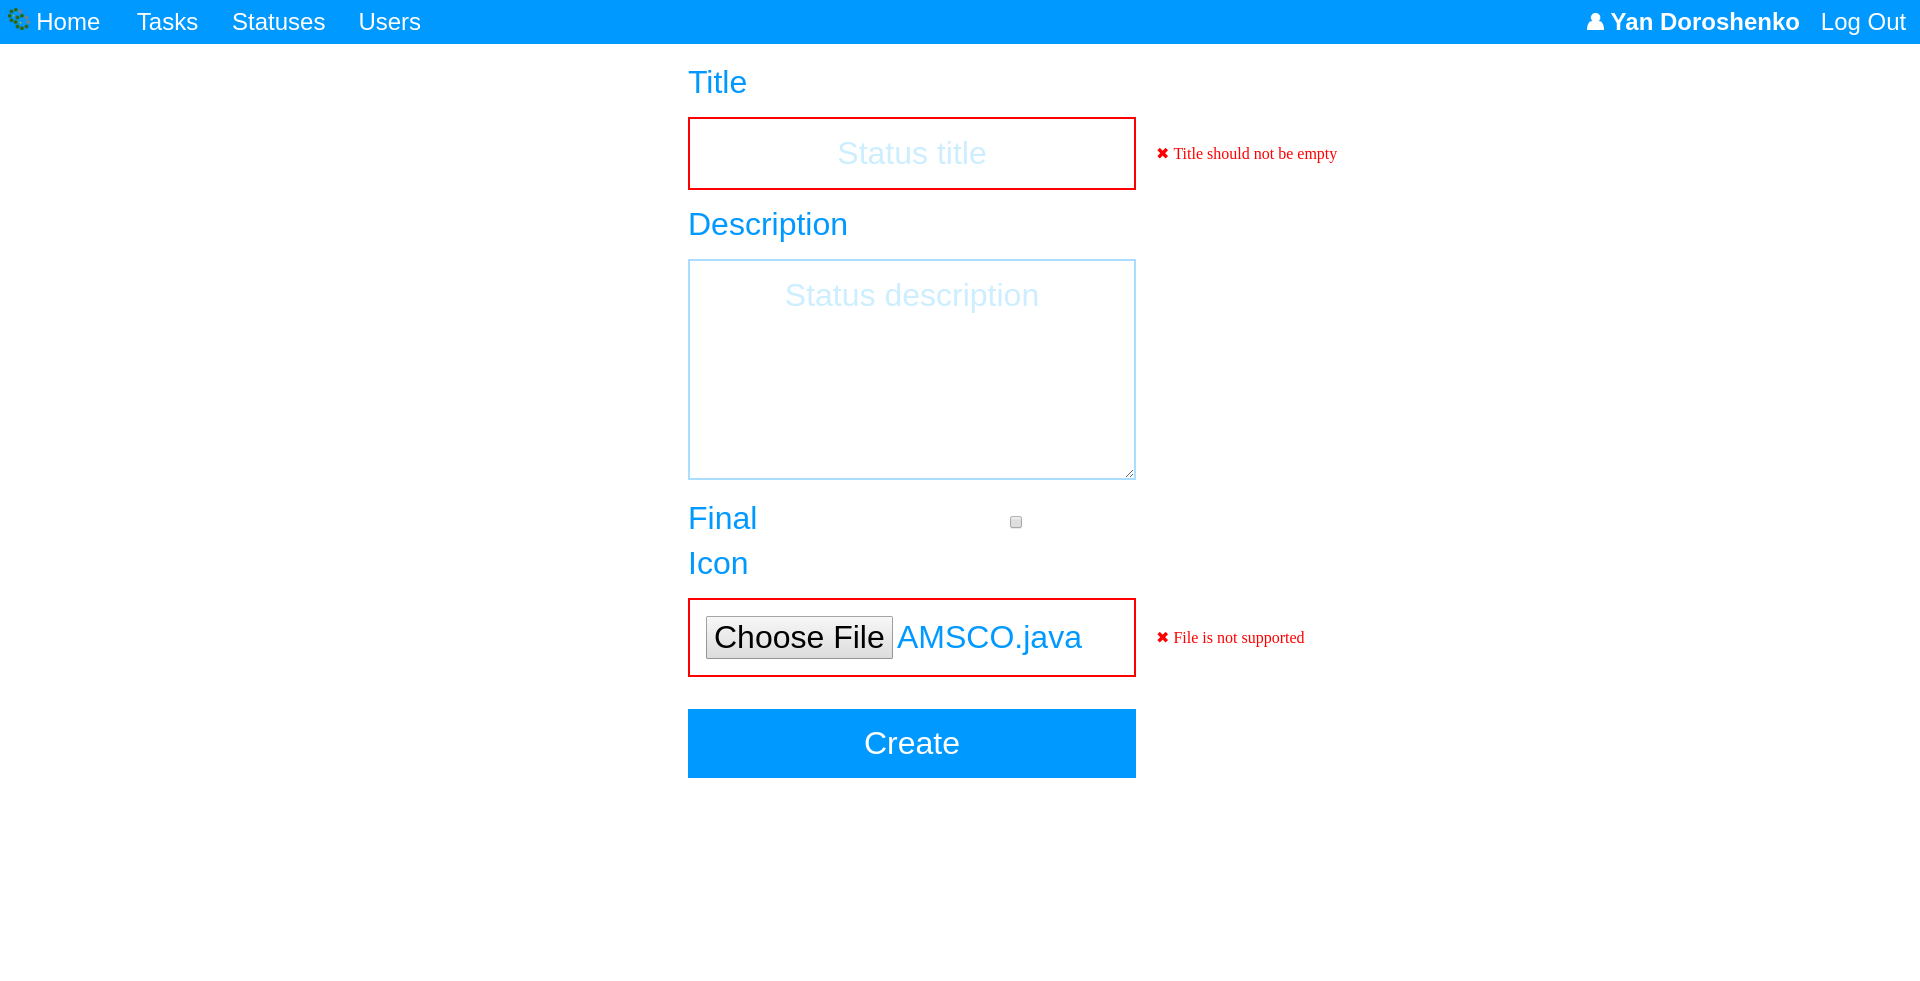
\includegraphics[width=\textwidth]{img/createstatus.png}
    \caption{Status creation page}
\end{figure}
\end{document}
